\chapter{Xray-Core Mathematics: Cryptographic Foundations and Protocol Design}

This chapter provides a deep mathematical and algorithmic analysis of Xray-core's cryptographic implementations. We explore stream ciphers, block ciphers, key exchange protocols, and reliable transport mechanisms with detailed mathematical formulations, TikZ diagrams, and code examples from the Xray-core source code.

\section{Introduction to Xray-Core Cryptography}

Xray-core implements multiple cryptographic primitives for secure proxy communication:
\begin{itemize}
    \item \textbf{Stream Ciphers}: ChaCha20 for high-performance encryption
    \item \textbf{Block Ciphers}: AES in multiple modes (CFB, CTR, GCM)
    \item \textbf{Key Exchange}: X25519 (Curve25519) and ML-KEM-768 for post-quantum security
    \item \textbf{AEAD}: Authenticated Encryption with Associated Data for integrity
    \item \textbf{Hash Functions}: FNV-1a, MD5, SHA-3, BLAKE3
    \item \textbf{Reliable Transport}: KCP protocol with sliding window algorithms
\end{itemize}

\section{ChaCha20 Stream Cipher}

ChaCha20 is a stream cipher designed by Daniel J. Bernstein, providing high performance and security. Xray-core implements ChaCha20 for efficient encryption of proxy traffic.

\subsection{Mathematical Foundation}

ChaCha20 operates on a 512-bit state organized as 16 words of 32 bits each. The state is initialized with:
\begin{itemize}
    \item 4 constant words: $c_0 = \texttt{0x61707865}$, $c_1 = \texttt{0x3320646e}$, $c_2 = \texttt{0x79622d32}$, $c_3 = \texttt{0x6b206574}$
    \item 8 key words: $k_0, k_1, \ldots, k_7$ (256-bit key)
    \item 4 nonce/counter words: $n_0, n_1, n_2, n_3$ (128-bit nonce + counter)
\end{itemize}

The initial state matrix is:
\[
S = \begin{bmatrix}
c_0 & c_1 & c_2 & c_3 \\
k_0 & k_1 & k_2 & k_3 \\
k_4 & k_5 & k_6 & k_7 \\
n_0 & n_1 & n_2 & n_3
\end{bmatrix}
\]

\subsection{Quarter-Round Operation}

ChaCha20 uses a quarter-round function $QR(a, b, c, d)$ that operates on four 32-bit words:
\begin{align}
a &\leftarrow a + b \\
d &\leftarrow (d \oplus a) \lll 16 \\
c &\leftarrow c + d \\
b &\leftarrow (b \oplus c) \lll 12 \\
a &\leftarrow a + b \\
d &\leftarrow (d \oplus a) \lll 8 \\
c &\leftarrow c + d \\
b &\leftarrow (b \oplus c) \lll 7
\end{align}

where $\lll$ denotes left rotation and $\oplus$ is XOR.

\begin{figure}[h]
    \centering
    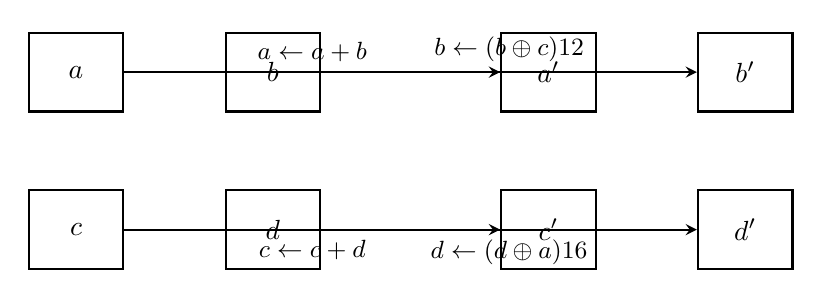
\begin{tikzpicture}[node distance=2cm,>=stealth,thick]
        \node (a1) [draw, rectangle, minimum width=1.2cm, minimum height=1cm] {$a$};
        \node (b1) [draw, rectangle, minimum width=1.2cm, minimum height=1cm, right of=a1, xshift=0.5cm] {$b$};
        \node (c1) [draw, rectangle, minimum width=1.2cm, minimum height=1cm, below of=a1] {$c$};
        \node (d1) [draw, rectangle, minimum width=1.2cm, minimum height=1cm, right of=c1, xshift=0.5cm] {$d$};
        
        \node (a2) [draw, rectangle, minimum width=1.2cm, minimum height=1cm, right of=b1, xshift=1.5cm] {$a'$};
        \node (b2) [draw, rectangle, minimum width=1.2cm, minimum height=1cm, right of=a2, xshift=0.5cm] {$b'$};
        \node (c2) [draw, rectangle, minimum width=1.2cm, minimum height=1cm, below of=a2] {$c'$};
        \node (d2) [draw, rectangle, minimum width=1.2cm, minimum height=1cm, right of=c2, xshift=0.5cm] {$d'$};
        
        \draw[->] (a1) -- node[above, font=\small] {$a \leftarrow a+b$} (a2);
        \draw[->] (b1) -- node[above, font=\small] {$b \leftarrow (b \oplus c) \lll 12$} (b2);
        \draw[->] (c1) -- node[below, font=\small] {$c \leftarrow c+d$} (c2);
        \draw[->] (d1) -- node[below, font=\small] {$d \leftarrow (d \oplus a) \lll 16$} (d2);
    \end{tikzpicture}
    \caption{ChaCha20 Quarter-Round Operation Flow}
\end{figure}

\subsection{ChaCha20 Block Function}

The ChaCha20 block function applies 20 rounds (10 double rounds) of column and diagonal mixing:

\begin{verbatim}
// From Xray-core: common/crypto/internal/chacha.go
func ChaCha20Block(state *[16]uint32, output []byte, rounds int) {
    working := *state  // Copy state
    
    // Column rounds (even rounds)
    for i := 0; i < rounds/2; i++ {
        QR(&working[0], &working[4], &working[8],  &working[12])  // Column 0
        QR(&working[1], &working[5], &working[9],  &working[13])  // Column 1
        QR(&working[2], &working[6], &working[10], &working[14])  // Column 2
        QR(&working[3], &working[7], &working[11], &working[15])  // Column 3
        
        // Diagonal rounds (odd rounds)
        QR(&working[0], &working[5], &working[10], &working[15])  // Diagonal 0
        QR(&working[1], &working[6], &working[11], &working[12])  // Diagonal 1
        QR(&working[2], &working[7], &working[8],  &working[13])  // Diagonal 2
        QR(&working[3], &working[4], &working[9],  &working[14])  // Diagonal 3
    }
    
    // Add original state (modular addition)
    for i := 0; i < 16; i++ {
        binary.LittleEndian.PutUint32(output[i*4:], working[i] + state[i])
    }
}
\end{verbatim}

The output keystream is computed as:
\[
\text{keystream} = S_{\text{initial}} + S_{\text{working}} \pmod{2^{32}}
\]

\subsection{ChaCha20 Stream Generation}

Xray-core generates a continuous keystream by incrementing the counter and generating new blocks:

\begin{verbatim}
// From Xray-core: common/crypto/internal/chacha.go
func (s *ChaCha20Stream) XORKeyStream(dst, src []byte) {
    i := 0
    max := len(src)
    for i < max {
        gap := blockSize - s.offset  // blockSize = 64 bytes
        
        limit := i + gap
        if limit > max {
            limit = max
        }
        
        // XOR with current block
        o := s.offset
        for j := i; j < limit; j++ {
            dst[j] = src[j] ^ s.block[o]
            o++
        }
        
        i += gap
        s.offset = o
        
        // Generate next block if needed
        if o == blockSize {
            s.offset = 0
            s.state[12]++  // Increment counter
            ChaCha20Block(&s.state, s.block[:], s.rounds)
        }
    }
}
\end{verbatim}

The encryption/decryption is simply:
\[
\text{ciphertext} = \text{plaintext} \oplus \text{keystream}
\]

\section{AES Encryption Modes}

Xray-core supports multiple AES modes: CFB (Cipher Feedback), CTR (Counter), and GCM (Galois/Counter Mode).

\subsection{AES-CFB (Cipher Feedback Mode)}

CFB mode turns AES into a stream cipher. The encryption process is:

\[
C_i = P_i \oplus E_K(S_i)
\]
\[
S_{i+1} = (S_i \ll 8) | C_i
\]

where $S_i$ is the shift register state, $P_i$ is plaintext, $C_i$ is ciphertext, and $E_K$ is AES encryption.

\begin{figure}[h]
    \centering
    \begin{tikzpicture}[node distance=4cm,>=stealth,thick]
        \node (iv) [draw, rectangle, minimum width=1.5cm, minimum height=1cm] {IV};
        \node (aes1) [draw, rectangle, right of=iv, minimum width=2cm, minimum height=1cm] {AES Encrypt};
        \node (xor1) [draw, circle, right of=aes1, minimum size=1cm] {$\oplus$};
        \node (c1) [draw, rectangle, right of=xor1, minimum width=1.5cm, minimum height=1cm] {$C_1$};
        \node (shift) [draw, rectangle, below of=aes1, minimum width=2cm, minimum height=1cm, yshift=-0.5cm] {Shift Register};
        \node (aes2) [draw, rectangle, right of=shift, minimum width=2cm, minimum height=1cm] {AES Encrypt};
        \node (xor2) [draw, circle, right of=aes2, minimum size=1cm] {$\oplus$};
        \node (c2) [draw, rectangle, right of=xor2, minimum width=1.5cm, minimum height=1cm] {$C_2$};
        
        \draw[->] (iv) -- (aes1);
        \draw[->] (aes1) -- node[above, font=\small] {$E_K(S_1)$} (xor1);
        \draw[->] (xor1) -- (c1);
        \draw[->] (c1) -- node[left, font=\small] {Shift} (shift);
        \draw[->] (shift) -- (aes2);
        \draw[->] (aes2) -- node[above, font=\small] {$E_K(S_2)$} (xor2);
        \draw[->] (xor2) -- (c2);
        
        \node (p1) [above of=xor1, yshift=-0.7cm] {$P_1$};
        \node (p2) [above of=xor2, yshift=-0.7cm] {$P_2$};
        \draw[->] (p1) -- (xor1);
        \draw[->] (p2) -- (xor2);
    \end{tikzpicture}
    \caption{AES-CFB Mode Encryption Flow}
\end{figure}

\subsection{AES-CTR (Counter Mode)}

CTR mode uses AES to generate a keystream from a counter:

\[
\text{keystream}_i = E_K(\text{nonce} || \text{counter}_i)
\]
\[
C_i = P_i \oplus \text{keystream}_i
\]

\begin{verbatim}
// From Xray-core: common/crypto/aes.go
func NewAesCTRStream(key []byte, iv []byte) cipher.Stream {
    return NewAesStreamMethod(key, iv, cipher.NewCTR)
}
\end{verbatim}

\subsection{AES-GCM (Galois/Counter Mode)}

GCM provides authenticated encryption. The encryption process:

\begin{enumerate}
    \item Generate keystream: $H = E_K(0^{128})$
    \item Encrypt: $C_i = P_i \oplus E_K(\text{IV} || i)$
    \item Compute authentication tag using GHASH:
    \[
    \text{Tag} = \text{GHASH}_H(\text{AAD} || C || \text{len}(AAD) || \text{len}(C))
    \]
\end{enumerate}

GHASH operates in $\text{GF}(2^{128})$:
\[
\text{GHASH}_H(X) = X_1 \cdot H \oplus X_2 \cdot H^2 \oplus \cdots \oplus X_n \cdot H^n
\]

\begin{verbatim}
// From Xray-core: common/crypto/aes.go
func NewAesGcm(key []byte) cipher.AEAD {
    block := common.Must2(aes.NewCipher(key))
    aead := common.Must2(cipher.NewGCM(block))
    return aead
}
\end{verbatim}

\section{VMess Protocol Authentication}

VMess uses time-based authentication with UUID and alterId. The authentication process involves:

\subsection{Time-Based Nonce Generation}

VMess requires system time to be synchronized within ±120 seconds of UTC. The authentication uses:

\[
\text{nonce} = \text{MD5}(\text{UUID} || \text{timestamp} || \text{alterId})
\]

where timestamp is the current UTC time in seconds.

\subsection{VMess Authentication Hash}

The authentication uses FNV-1a hash function:

\begin{verbatim}
// From Xray-core: proxy/vmess/encoding/auth.go
func Authenticate(b []byte) uint32 {
    fnv1hash := fnv.New32a()
    common.Must2(fnv1hash.Write(b))
    return fnv1hash.Sum32()
}
\end{verbatim}

FNV-1a hash algorithm:
\[
\text{hash} = \text{FNV\_OFFSET\_BASIS}
\]
\[
\text{for each byte } b: \text{hash} = (\text{hash} \oplus b) \cdot \text{FNV\_PRIME} \pmod{2^{32}}
\]

where $\text{FNV\_OFFSET\_BASIS} = 2166136261$ and $\text{FNV\_PRIME} = 16777619$.

\subsection{ChaCha20-Poly1305 Key Derivation}

VMess derives ChaCha20-Poly1305 keys using MD5:

\begin{verbatim}
// From Xray-core: proxy/vmess/encoding/auth.go
func GenerateChacha20Poly1305Key(b []byte) []byte {
    key := make([]byte, 32)
    t := md5.Sum(b)
    copy(key, t[:])           // First 16 bytes: MD5(b)
    t = md5.Sum(key[:16])
    copy(key[16:], t[:])       // Second 16 bytes: MD5(MD5(b))
    return key
}
\end{verbatim}

Mathematically:
\[
K[0:16] = \text{MD5}(b)
\]
\[
K[16:32] = \text{MD5}(K[0:16])
\]

\section{VLESS Encryption and Key Exchange}

VLESS uses advanced key exchange mechanisms including X25519 (Curve25519) and ML-KEM-768 for post-quantum security.

\subsection{Curve25519 Key Exchange}

Curve25519 is an elliptic curve over $\mathbb{F}_{2^{255}-19}$ defined by:
\[
y^2 = x^3 + 486662x^2 + x
\]

The base point $G$ has order $8\ell$ where $\ell$ is a large prime. The key exchange:

\begin{enumerate}
    \item Client generates private key: $a \in_R [0, 2^{256})$
    \item Client computes public key: $A = aG$
    \item Server has public key: $B$
    \item Shared secret: $S = aB = abG$
    \item Derived key: $K = \text{BLAKE3}(S)$
\end{enumerate}

\begin{verbatim}
// From Xray-core: proxy/vless/encryption/client.go
privateKey, _ := ecdh.X25519().GenerateKey(rand.Reader)
nfsKey, err := privateKey.ECDH(serverPublicKey)
if err != nil {
    return nil, err
}
\end{verbatim}

\subsection{ML-KEM-768 Post-Quantum Key Exchange}

ML-KEM-768 (Module-Lattice Key Encapsulation Mechanism) provides post-quantum security:

\begin{enumerate}
    \item Server generates key pair: $(sk, pk) = \text{ML-KEM-768.KeyGen}()$
    \item Client encapsulates: $(K, ct) = \text{ML-KEM-768.Encaps}(pk)$
    \item Server decapsulates: $K' = \text{ML-KEM-768.Decaps}(sk, ct)$
    \item Shared key: $K = K'$ (with high probability)
\end{enumerate}

\begin{verbatim}
// From Xray-core: proxy/vless/encryption/client.go
if k, ok := k.(*mlkem.EncapsulationKey768); ok {
    var ciphertext []byte
    nfsKey, ciphertext = k.Encapsulate()
    copy(relays, ciphertext)  // 1088 bytes
    index = 1088
}
\end{verbatim}

\subsection{VLESS United Key Derivation}

VLESS combines multiple key exchange results:

\[
\text{UnitedKey} = \text{PFSKey} || \text{NFSKey}
\]

where PFSKey is derived from ML-KEM-768 + X25519, and NFSKey is from the relay chain.

\begin{verbatim}
// From Xray-core: proxy/vless/encryption/client.go
pfsKey := make([]byte, 32+32)  // ML-KEM-768 (32) + X25519 (32)
copy(pfsKey, mlkem768Key)
copy(pfsKey[32:], x25519Key)
c.UnitedKey = append(pfsKey, nfsKey...)
\end{verbatim}

\section{KCP Protocol: Reliable Transport Mathematics}

KCP (A Fast and Reliable ARQ Protocol) implements a sliding window protocol with adaptive retransmission.

\subsection{Sliding Window Algorithm}

KCP maintains a sending window and receiving window. The sending window tracks unacknowledged segments:

\[
\text{WindowSize} = \min(\text{CongestionWindow}, \text{ReceiveWindow})
\]

\subsection{RTT Estimation}

KCP uses exponential weighted moving average (EWMA) for RTT estimation:

\[
\text{RTT} = \alpha \cdot \text{RTT}_{\text{old}} + (1-\alpha) \cdot \text{RTT}_{\text{sample}}
\]

where $\alpha$ is typically 0.7.

\subsection{Retransmission Timeout (RTO)}

RTO is calculated using RTT and RTT variance:

\[
\text{RTO} = \text{RTT} + 4 \cdot \text{RTTVar}
\]

\begin{verbatim}
// From Xray-core: transport/internet/kcp/segment.go
type DataSegment struct {
    Conv        uint16
    Option      SegmentOption
    Timestamp   uint32      // Send timestamp
    Number      uint32      // Sequence number
    SendingNext uint32     // Next expected ACK
    payload     *buf.Buffer
    timeout     uint32      // Retransmission timeout
    transmit    uint32      // Transmission count
}
\end{verbatim}

\subsection{Fast Retransmit}

KCP implements fast retransmit when duplicate ACKs are received:

\[
\text{if } \text{dupACKs} \geq 3: \text{retransmit immediately}
\]

\begin{figure}[h]
    \centering
    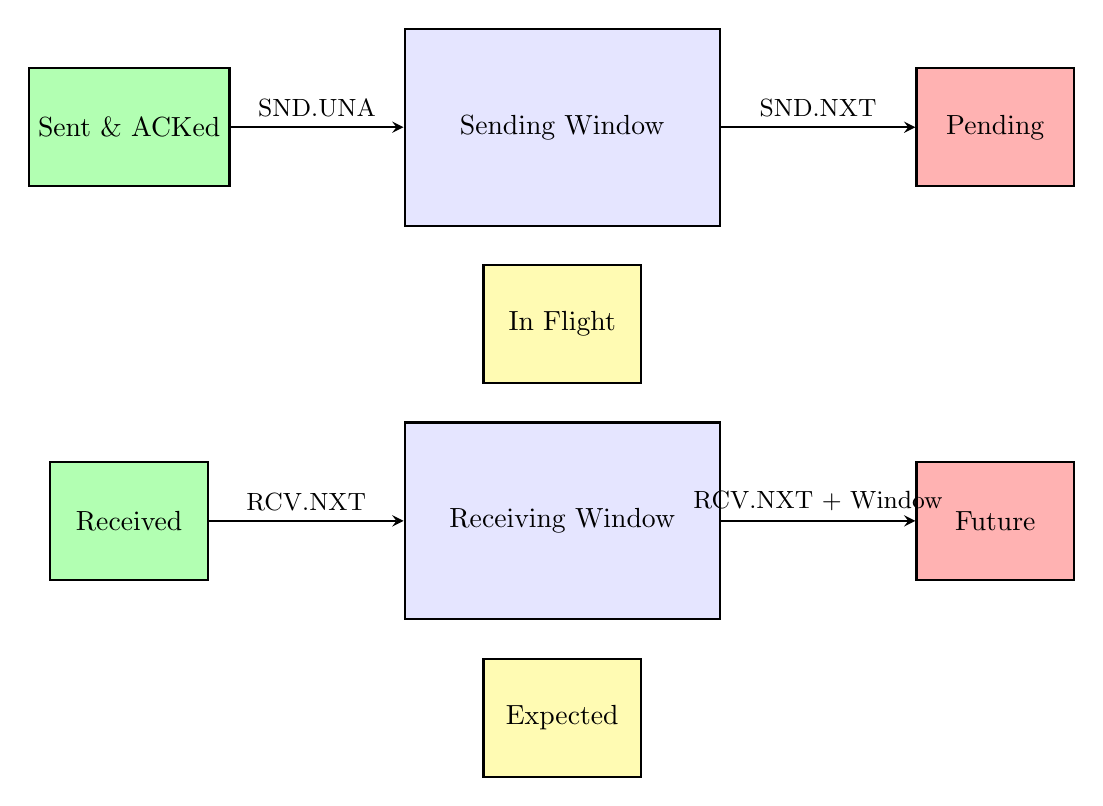
\begin{tikzpicture}[node distance=3cm,>=stealth,thick]
        \node (sw) [draw, rectangle, minimum width=4cm, minimum height=2.5cm, fill=blue!10] {Sending Window};
        \node (sent) [draw, rectangle, left of=sw, xshift=-2.5cm, fill=green!30, minimum width=2cm, minimum height=1.5cm] {Sent \& ACKed};
        \node (inflight) [draw, rectangle, fill=yellow!30, minimum width=2cm, minimum height=1.5cm, below of=sw, yshift=0.5cm] {In Flight};
        \node (pending) [draw, rectangle, right of=sw, xshift=2.5cm, fill=red!30, minimum width=2cm, minimum height=1.5cm] {Pending};
        
        \draw[->, thick] (sent) -- node[above, font=\small] {SND.UNA} (sw);
        \draw[->, thick] (sw) -- node[above, font=\small] {SND.NXT} (pending);
        
        \node (rw) [draw, rectangle, minimum width=4cm, minimum height=2.5cm, below of=sw, yshift=-2cm, fill=blue!10] {Receiving Window};
        \node (received) [draw, rectangle, left of=rw, xshift=-2.5cm, fill=green!30, minimum width=2cm, minimum height=1.5cm] {Received};
        \node (expected) [draw, rectangle, fill=yellow!30, minimum width=2cm, minimum height=1.5cm, below of=rw, yshift=0.5cm] {Expected};
        \node (future) [draw, rectangle, right of=rw, xshift=2.5cm, fill=red!30, minimum width=2cm, minimum height=1.5cm] {Future};
        
        \draw[->, thick] (received) -- node[above, font=\small] {RCV.NXT} (rw);
        \draw[->, thick] (rw) -- node[above, font=\small] {RCV.NXT + Window} (future);
    \end{tikzpicture}
    \caption{KCP Sliding Window Protocol}
\end{figure}

\section{Shadowsocks Encryption}

Shadowsocks uses stream ciphers with key derivation from password.

\subsection{Key Derivation}

Shadowsocks derives encryption keys using HKDF (HMAC-based Key Derivation Function):

\[
\text{Key} = \text{HKDF-Expand}(\text{HKDF-Extract}(\text{salt}, \text{password}), \text{info}, \text{length})
\]

\begin{verbatim}
// From Xray-core: proxy/shadowsocks/config.go
func (a *Account) getCipher() (Cipher, error) {
    switch a.CipherType {
    case CipherType_AES_128_GCM:
        return &AEADCipher{
            KeyBytes: 16,
            IVBytes:  16,
            AEAD:     createAesGcm,
        }, nil
    case CipherType_CHACHA20_POLY1305:
        return &AEADCipher{
            KeyBytes: 32,
            IVBytes:  12,
            AEAD:     createChaCha20Poly1305,
        }, nil
    }
}
\end{verbatim}

\subsection{IV Generation and Anti-Replay}

Shadowsocks uses unique IVs to prevent replay attacks:

\[
\text{IV} \in_R \{0,1\}^{128} \text{ (for AES-GCM)}
\]

The anti-replay filter checks:
\[
\text{if } \text{IV} \in \text{ReplayFilter}: \text{reject}
\]

\begin{verbatim}
// From Xray-core: proxy/shadowsocks/config.go
func (a *MemoryAccount) CheckIV(iv []byte) error {
    if a.replayFilter == nil {
        return nil
    }
    if a.replayFilter.Check(iv) {
        return nil  // IV is unique
    }
    return ErrIVNotUnique
}
\end{verbatim}

\section{AEAD: Authenticated Encryption with Associated Data}

AEAD provides both confidentiality and authenticity. Xray-core implements AEAD for multiple protocols.

\subsection{AEAD Encryption Process}

The encryption process:
\[
(C, \text{Tag}) = \text{AEAD.Seal}(\text{nonce}, \text{plaintext}, \text{AAD})
\]

where:
\begin{itemize}
    \item $C$ is the ciphertext
    \item $\text{Tag}$ is the authentication tag
    \item $\text{AAD}$ is additional authenticated data (not encrypted)
\end{itemize}

\subsection{AEAD Decryption and Verification}

The decryption process:
\[
(P, \text{valid}) = \text{AEAD.Open}(\text{nonce}, C, \text{AAD})
\]

If $\text{valid} = \text{false}$, the ciphertext is rejected.

\begin{verbatim}
// From Xray-core: common/crypto/auth.go
func (v *AEADAuthenticator) Seal(dst, plainText []byte) ([]byte, error) {
    iv := v.NonceGenerator()
    var additionalData []byte
    if v.AdditionalDataGenerator != nil {
        additionalData = v.AdditionalDataGenerator()
    }
    return v.AEAD.Seal(dst, iv, plainText, additionalData), nil
}

func (v *AEADAuthenticator) Open(dst, cipherText []byte) ([]byte, error) {
    iv := v.NonceGenerator()
    var additionalData []byte
    if v.AdditionalDataGenerator != nil {
        additionalData = v.AdditionalDataGenerator()
    }
    return v.AEAD.Open(dst, iv, cipherText, additionalData)
}
\end{verbatim}

\subsection{Nonce Generation Strategies}

Xray-core supports multiple nonce generation strategies:

\begin{enumerate}
    \item \textbf{Increasing Nonce}: Counter-based, increments for each encryption
    \[
    \text{nonce}_i = \text{nonce}_0 + i
    \]
    
    \item \textbf{Random Nonce}: Cryptographically random for each encryption
    \[
    \text{nonce}_i \in_R \{0,1\}^{96}
    \]
\end{enumerate}

\begin{verbatim}
// From Xray-core: common/crypto/auth.go
func GenerateIncreasingNonce(nonce []byte) BytesGenerator {
    c := append([]byte(nil), nonce...)
    return func() []byte {
        for i := range c {
            c[i]++
            if c[i] != 0 {
                break
            }
        }
        return c
    }
}
\end{verbatim}

\section{KCP Simple Authenticator}

KCP uses a lightweight authenticator for legacy compatibility:

\subsection{FNV Hash Authentication}

The simple authenticator uses FNV-32a hash:

\begin{verbatim}
// From Xray-core: transport/internet/kcp/crypt.go
func (a *SimpleAuthenticator) Seal(dst, nonce, plain, extra []byte) []byte {
    dst = append(dst, 0, 0, 0, 0, 0, 0)  // 4 bytes hash + 2 bytes length
    binary.BigEndian.PutUint16(dst[4:], uint16(len(plain)))
    dst = append(dst, plain...)
    
    fnvHash := fnv.New32a()
    common.Must2(fnvHash.Write(dst[4:]))  // Hash length + plaintext
    fnvHash.Sum(dst[:0])                   // Write hash to first 4 bytes
    
    // XOR obfuscation
    xtra := 4 - len(dst)%4
    if xtra != 4 {
        dst = append(dst, make([]byte, xtra)...)
    }
    xorfwd(dst)  // Forward XOR
    if xtra != 4 {
        dst = dst[:len(dst)-xtra]
    }
    return dst
}
\end{verbatim}

The authentication tag is:
\[
\text{Tag} = \text{FNV-32a}(\text{length} || \text{plaintext})
\]

\subsection{XOR Obfuscation}

KCP applies XOR obfuscation to make traffic patterns less distinguishable:

\[
\text{for } i = 0 \text{ to } n-1: \text{data}[i] = \text{data}[i] \oplus \text{data}[(i+1) \bmod n]
\]

\section{Hash Functions in Xray-Core}

Xray-core uses multiple hash functions for different purposes:

\subsection{BLAKE3}

BLAKE3 is used for key derivation in VLESS:

\[
K = \text{BLAKE3}(\text{publicKey})
\]

BLAKE3 uses a Merkle tree structure:
\[
\text{BLAKE3}(M) = \text{Compress}(\text{Chunk}_0 || \text{Chunk}_1 || \cdots || \text{Chunk}_n)
\]

\begin{verbatim}
// From Xray-core: proxy/vless/encryption/client.go
i.Hash32s[j] = blake3.Sum256(k)  // 32-byte hash of public key
\end{verbatim}

\subsection{SHA-3 (SHAKE)}

SHAKE-128 is used for size parser in VMess:

\[
\text{mask} = \text{SHAKE-128}(\text{nonce})
\]
\[
\text{encryptedSize} = \text{size} \oplus \text{mask}[0:2]
\]

\begin{verbatim}
// From Xray-core: proxy/vmess/encoding/auth.go
func NewShakeSizeParser(nonce []byte) *ShakeSizeParser {
    shake := sha3.NewShake128()
    common.Must2(shake.Write(nonce))
    return &ShakeSizeParser{shake: shake}
}

func (s *ShakeSizeParser) Encode(size uint16, b []byte) []byte {
    mask := s.next()  // Get 2 bytes from SHAKE-128 stream
    binary.BigEndian.PutUint16(b, mask^size)
    return b[:2]
}
\end{verbatim}

\section{Summary}

This chapter covered the mathematical foundations of Xray-core's cryptographic implementations:

\begin{itemize}
    \item \textbf{ChaCha20}: Stream cipher with 20-round block function and quarter-round operations
    \item \textbf{AES}: Multiple modes (CFB, CTR, GCM) for different security and performance requirements
    \item \textbf{VMess}: Time-based authentication with FNV hash and ChaCha20-Poly1305
    \item \textbf{VLESS}: Advanced key exchange with X25519 and ML-KEM-768 for post-quantum security
    \item \textbf{KCP}: Sliding window protocol with adaptive RTT estimation and fast retransmit
    \item \textbf{Shadowsocks}: HKDF-based key derivation with AEAD encryption
    \item \textbf{AEAD}: Authenticated encryption providing confidentiality and integrity
    \item \textbf{Hash Functions}: BLAKE3, SHA-3, FNV-1a for various cryptographic purposes
\end{itemize}

Understanding these mathematical foundations is essential for:
\begin{itemize}
    \item Debugging cryptographic issues
    \item Optimizing performance
    \item Implementing protocol extensions
    \item Ensuring security properties
\end{itemize}

\section{Further Reading}

\begin{itemize}
    \item ChaCha20 and Poly1305: \url{https://tools.ietf.org/html/rfc8439}
    \item AES-GCM: \url{https://nvlpubs.nist.gov/nistpubs/Legacy/SP/nistspecialpublication800-38d.pdf}
    \item Curve25519: \url{https://cr.yp.to/ecdh.html}
    \item ML-KEM: \url{https://csrc.nist.gov/publications/detail/fips/203/final}
    \item KCP Protocol: \url{https://github.com/skywind3000/kcp}
    \item BLAKE3: \url{https://github.com/BLAKE3-team/BLAKE3}
\end{itemize}

